% ============================================================
% 4. RoLA
%
% Every equation is verified against
% ROLA_HIERARCHICAL_VALUE_MEMORY_ARCHITECTURE.md rev 2026-07-29.18, which is
% normative for the model mathematics:
%   Eq. (1),(2)  <- arch 4.1 (topology, allocations, level configurations)
%   Eq. (3)      <- arch 4.2 (one mass per side; leaf factors)
%   Eq. (4),(5)  <- arch 4.3 (value recurrence, num/den/readout; the epsilon
%                  convention, here written eta so that epsilon stays free for
%                  the union error carried into Sec. 7)
%   Eq. (6)      <- arch 4.4.2 LeafMassDecay (compact per-branch dials, the
%                  AND-product leaf rate, the detached clock, g_write absent
%                  from the clock, strict complete-leaf immortality)
%   Eq. (7)      <- the touch product, r*w = prod_l b_l = N. SCOPED: it governs
%                  the ALL-COVERAGE wirings only (every level dense on exactly
%                  one side); r and w are STRUCTURAL ENVELOPES, guarantee
%                  widths and not per-token bills, the realized entmax support
%                  sitting at or below them; the shared solve sits at r*w << N
%                  by design. Ratified form recovered from Sec. 7 at ee169ee.
%                  Never write that a token touches r and w, and never state
%                  the product without naming the all-coverage scope.
%   Eq. (8)      <- union split, settled source semantics:
%                  p = entmax((z_r + z_w)/2), sigma = sigmoid(z_r - z_w),
%                  read = p*sigma UNNORMALIZED, write = p*(1-sigma)
%                  RENORMALIZED over supp(p). The AVERAGE (not the sum) is the
%                  settled form (user decision 2026-07-11, recorded in
%                  rola-scratch/workflows/union-split/findings.txt under
%                  "AVERAGE CORRECTION"); rola_bench/named_configs.py still
%                  quotes the superseded sum form in its docstring and is stale
%                  on this point. Re-verified against
%                  rola-standalone/rola/routing/reference.py
%                  (_union_split_with_support).
% WIRING BLOCK (user-ratified restructure, 2026-08-03): the legacy stratification
% is dissolved. sec:wiring "Structural requirements" states the constraint system
% once (single-mechanism premise, the trainability guarantee and the wiring it
% excludes, agreement-or-coverage, the touch pricing of Eq. (7)) and carries NO
% candidate detail. Tab. wirings is the hinge, the derivation's output, placed
% between the requirements and the candidates. Then one small structurally
% parallel subsection per candidate, each in the same internal shape
% (construction, how it buys the guarantee, classification, liability):
% sec:denseread, sec:levelsides, sec:union. The old "The shared-support solve"
% subsection dissolved into sec:union under that shape, and the third-geometry
% paragraph that used to close it became sec:levelsides. One home per sentence:
% Sec. 7 re-contextualizes and states no law sentence of its own.
%
% Capacity claims belong to Sec. 5 and cost claims to Sec. 6; this section
% cross-references both and states neither.
% ============================================================
\section{RoLA}
\label{sec:rola}

This section fixes the head the reduction licenses. A RoLA head keeps a state of $\Nst$ features, and its feature map gives each token key features saying which it writes and query features saying which it reads. Four parts are configurable, and the subsections below fix each: the level configuration, the activation each allocation comes from, the decay semantics, and the readout normalization. Allocations stay normalized and nonnegative, the regime scoped in Section~\ref{sec:reduction}.

\subsection{Topology of the feature map}
\label{sec:topology}

The map is a hierarchy of levels whose complete addresses are its features. Fix one batch element and one head. The map has $\Dlv$ levels, level $l$ of branch width $\bl$. A leaf address picks one branch per level, and the feature count is the product of the widths:
\begin{align}
  s = (d_0, \dots, d_{\Dlv-1}), \qquad d_l \in \{1,\dots,\bl\},
  \qquad \Nst \;=\; \prod_{l=0}^{\Dlv-1} \bl ,
  \label{eq:leafcount}
\end{align}
one feature per leaf. We write $d_l(s)$ for the branch leaf $s$ takes at level $l$, and $\Slv = \sum_l \bl$ for the total branch width. The sum is what a side emits, the product is what it addresses, and the gap is what depth buys. The levels are scales of the address, where log-linear attention makes its hierarchy over the sequence axis \citep{guo2025loglinear}. A coarse level here selects a region of one fixed state, and every token passes through every level.

At token $t$ each side emits one allocation per level, a distribution over that level's branches saying where the side points:
\begin{align}
  p^{\mathrm{r}}_{l,t,d} \ge 0,\quad \textstyle\sum_d p^{\mathrm{r}}_{l,t,d} = 1,
  \qquad
  p^{\mathrm{w}}_{l,t,d} \ge 0,\quad \textstyle\sum_d p^{\mathrm{w}}_{l,t,d} = 1,
  \label{eq:levelalloc}
\end{align}
with $p^{\mathrm{r}}$ the read allocation and $p^{\mathrm{w}}$ the write allocation. Each level and side carries its own activation. Softmax is dense, while the $\alpha$-entmax family returns true zeros \citep{peters2019sparse, martins2016sparsemax}, meaning that a branch left out gets a true zero and not merely a small number. We use its order-$1.5$ member and sparsemax at order $2$.

The support of such a solve is the set of branches it puts mass on, in other words the branches the side actually touches. Everything else gets a true zero. That support has a boundary moving continuously with the logits, so the task gradient recruits and releases branches. We write $\entmaxop$ for whichever order a level carries, and reserve $\alpha$ for the provisioning ratio of Section~\ref{sec:capacity}.

Each level carries one of two configurations, independent or tied, and a tied level is what the shared-support solve of Section~\ref{sec:union} builds on (Appendix~\ref{apd:wirings}).

\begin{figure}[H]
\centering
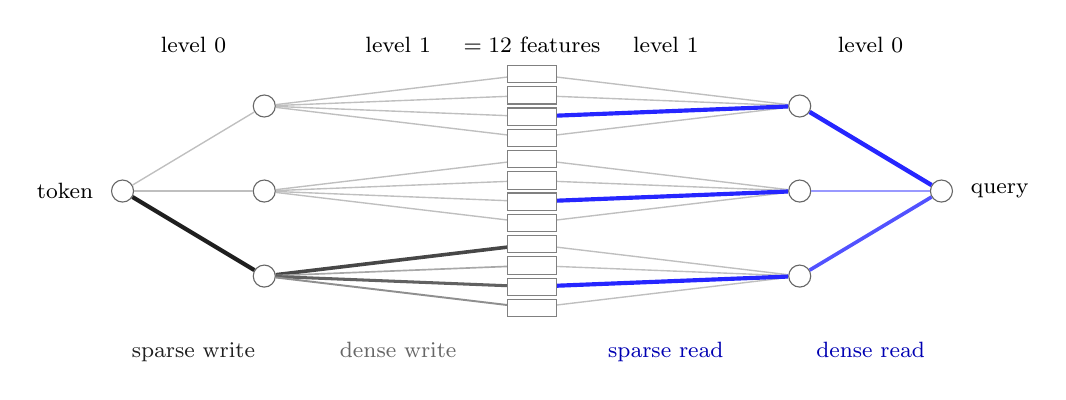
\begin{tikzpicture}[
  lf/.style={draw=black!50, fill=white, minimum width=0.62cm, minimum height=0.22cm, inner sep=0pt},
  nd/.style={draw=black!60, circle, inner sep=1pt, minimum size=0.28cm, fill=white},
  sk/.style={draw=black!25, line width=0.5pt},
  lb/.style={font=\footnotesize},
]
% Horizontal bowtie. The writing token enters at the left and routes through
% its levels into the leaf column; the query enters at the right and routes
% through the same levels into the same column. One distribution per level
% (Eq. 2), so level 1's pattern repeats under every level-0 branch.
% Drawn is the LEVEL SPLIT, the paper's one exported name for this wiring (Sec. 7,
% Tab. 5, App. A). "Split assignment" was an alias for it and is retired
% (settlement fix 2026-08-03: the alias is gone from this caption). The term
% is quarantined out of Sec. 4's prose (style gate B6), which states the geometry
% rather than naming it, so no gloss is owed here; the caption identifies the
% wiring by tab:wirings' own row phrase, "sparsity split by level". Level 0 writes sparsely and reads
% densely, level 1 writes densely and reads sparsely. Bold marks a sparse
% support and graded tint a dense one, black the write side and blue the read.
\foreach \i in {1,...,12}{\coordinate (p\i) at (0,{1.485-0.27*(\i-1)});}
\node[nd] (w1) at (-3.4,1.08) {}; \node[nd] (w2) at (-3.4,0) {}; \node[nd] (w3) at (-3.4,-1.08) {};
\node[nd] (r1) at ( 3.4,1.08) {}; \node[nd] (r2) at ( 3.4,0) {}; \node[nd] (r3) at ( 3.4,-1.08) {};
\node[nd] (tk) at (-5.2,0) {};    \node[nd] (qy) at ( 5.2,0) {};
% write side: sparse at level 0 (one branch, bold), dense at level 1 (tint)
\draw[sk] (tk)--(w1); \draw[sk] (tk)--(w2);
\draw[draw=black!88, line width=1.5pt] (tk)--(w3);
\foreach \j in {1,2,3,4}{\draw[sk] (w1)--(p\j);}
\foreach \j in {5,6,7,8}{\draw[sk] (w2)--(p\j);}
\foreach \j/\w/\o in {9/1.3/72, 10/0.6/34, 11/1.1/62, 12/0.7/44}{
  \draw[draw=black!\o!white, line width=\w pt] (w3)--(p\j);}
% read side: dense at level 0 (tint), sparse at level 1 (one branch each, bold)
\foreach \n/\w/\o in {r1/1.6/85, r2/0.7/40, r3/1.3/68}{
  \draw[draw=blue!\o!white, line width=\w pt] (qy)--(\n);}
\foreach \n/\j in {r1/1, r1/2, r1/4, r2/5, r2/6, r2/8, r3/9, r3/10, r3/12}{
  \draw[sk] (\n)--(p\j);}
\foreach \n/\j in {r1/3, r2/7, r3/11}{
  \draw[draw=blue!85!white, line width=1.5pt] (\n)--(p\j);}
\foreach \i in {1,...,12}{\node[lf] at (p\i) {};}
\node[lb, anchor=east] at (-5.45,0) {token};
\node[lb, anchor=west] at ( 5.45,0) {query};
\node[lb] at (-4.30,1.86) {level $0$};
\node[lb] at (-1.70,1.86) {level $1$};
\node[lb] at ( 0.00,1.86) {$\Nst = 12$ features};
\node[lb] at ( 1.70,1.86) {level $1$};
\node[lb] at ( 4.30,1.86) {level $0$};
\node[lb, anchor=north, black!88] at (-4.30,-1.80) {sparse write};
\node[lb, anchor=north, black!60] at (-1.70,-1.80) {dense write};
\node[lb, anchor=north, blue!70!black] at ( 1.70,-1.80) {sparse read};
\node[lb, anchor=north, blue!70!black] at ( 4.30,-1.80) {dense read};
\end{tikzpicture}
\caption{\textbf{The RoLA head.} Widths $b_0 = 3$ and $b_1 = 4$ give $\Nst = 12$ features, one per leaf address, and that column is the state. The token enters at the left and its query at the right, each passing through the same levels, so level 1's pattern repeats under every level-0 branch. A support drawn bold is sparse and one drawn as graded tint dense, black for the write side and blue for the read, each level assigning the two sides independently. The default configuration is sparse writes and dense reads at every level; drawn here is the sparsity split by level, sparse on the write at level 0 and on the read at level 1, which Section~\ref{sec:experiments} measures.}
\label{fig:head}
\end{figure}

\subsection{Allocation and mass}
\label{sec:allocation}

A write into a leaf carries three jobs, and normalizing the allocation keeps them apart. The allocation says where, one positive scalar per side per token, $g^{\mathrm{r}}_t$ and $g^{\mathrm{w}}_t$, says how much, and the value says what. The gain is the one of the three that reaches the mass alone, which is what makes it identifiable.

Halving the write gain and doubling the value leaves the numerator of the readout below where it was and halves the denominator. The item's weight against everything else the state holds moves, and the output moves with it. Proposition~\ref{prop:identity} carries $g^{\mathrm{w}}_t$ explicitly for that reason. The three jobs give leaf factors
\begin{align}
  R_{t,s} \;=\; g^{\mathrm{r}}_t \prod_{l} p^{\mathrm{r}}_{l,t,d_l(s)},
  \qquad
  W_{t,s} \;=\; g^{\mathrm{w}}_t \prod_{l} p^{\mathrm{w}}_{l,t,d_l(s)} ,
  \label{eq:leaffactors}
\end{align}
with $R_{t,s}$ and $W_{t,s}$ the weights leaf $s$ receives in the read and in the write. Both gains are token-conditioned.

Each side carries one mass and no more, per-level masses collapsing into a side-wide product (Appendix~\ref{apd:wirings}).

\subsection{The value recurrence}
\label{sec:recurrence}

Each leaf owns one value vector $M_{t,s} \in \R^{\dv}$, with $\dv$ the value width. A token deposits its projected value $v_t \in \R^{\dv}$ into every leaf its write factor reaches. Earlier contents survive by a factor $\mathrm{keep}_{t,s} \in (0,1]$ fixed in Section~\ref{sec:decay}, and the read contracts the state:
\begin{align}
  M_{t,s} \;=\; \mathrm{keep}_{t,s}\, M_{t-1,s} \;+\; W_{t,s}\, v_t ,
  \qquad
  \mathrm{num}_t \;=\; \textstyle\sum_{s} R_{t,s}\, M_{t,s} .
  \label{eq:recurrence}
\end{align}
The deposit is additive with input-dependent coefficients, so the recurrence is affine in the state, as Proposition~\ref{prop:reduction} asks.

Each leaf also carries a scalar mass $z_{t,s}$ under the same recurrence, and the readout divides the two contractions:
\begin{align}
  z_{t,s} = \mathrm{keep}_{t,s}\, z_{t-1,s} + W_{t,s},
  \qquad
  \mathrm{den}_t = \textstyle\sum_s R_{t,s}\, z_{t,s},
  \qquad
  y_t = \frac{\mathrm{num}_t}{\mathrm{den}_t + \eta} ,
  \label{eq:global}
\end{align}
with $\eta > 0$ a small constant. The mass is an appended constant-one value channel, and the read gain cancels between numerator and denominator, so we fix $g^{\mathrm{r}}_t = 1$.

The normalized readout has a consequence the rest of the paper leans on. A feature never written contributes zero to $\mathrm{num}_t$ and zero to $\mathrm{den}_t$. Reading it returns nothing rather than noise, so the write support need not contain the read support for correctness, which is what makes the sparse-write, dense-read topology safe.

\subsection{Decay on a write-mass clock}
\label{sec:decay}

With decay disabled, $\mathrm{keep}_{t,s} = 1$ and Eq.~\eqref{eq:recurrence} is additive. The learned form ages a feature by how much it has taken in, not by how long it has existed. In effect, a feature that nothing writes to keeps what it holds indefinitely. Each level carries a per-branch dial $\delta_{l,d} \in [0,1)$, and a leaf's rate is the product of the dials on its own address. The exponent is the write mass that leaf receives at this token, held off the gradient by a stop-gradient $\mathrm{sg}[\cdot]$:
\begin{align}
  w^{\mathrm{leaf}}_{t,s} = \prod_{l} p^{\mathrm{w}}_{l,t,d_l(s)},
  \qquad
  \mathrm{rate}_s = \prod_{l} \delta_{l, d_l(s)},
  \qquad
  \mathrm{keep}_{t,s} = \left( 1 - \mathrm{rate}_s \right)^{\mathrm{sg}[ w^{\mathrm{leaf}}_{t,s} ]} .
  \label{eq:decay}
\end{align}
The write gain $g^{\mathrm{w}}_t$ scales the deposit but stays out of the clock, which keeps the exponent in $[0,1]$.

The clock ignores that gain by design, since a state-dependent share of the accumulated mass would cross the input-affine boundary of Section~\ref{sec:reduction} (Appendix~\ref{apd:clock}).

In the gated linear-attention lineage the clock advances once per timestep, so a feature ages even when it takes no write \citep{yang2024gla, gu2023mamba, yang2024gdn, qin2024hgrn2}. Here an unwritten feature keeps every bit, which is the law we want once Section~\ref{sec:capacity} sizes the state so that almost every feature is idle at almost every step (Appendix~\ref{apd:clock}).

Forgetting in proportion to writing rather than to elapsed time is prior art and we do not claim it, RAM-Net's clock being the closest and Section~\ref{sec:reduction} the carve-out. Raven gates decay on selection \citep{afzal2026raven}, and usage-driven reallocation goes back to the differentiable-memory line \citep{graves2016dnc, rae2016sam}. Two properties of Eq.~\eqref{eq:decay} are ours.

The model learns the rate per level and composes it across the hierarchy. A leaf's rate comes from its own address, at $\Slv$ parameters, so a coarse region can stay durable while the features beneath it turn over.

The clock also runs detached. The stop-gradient leaves the recurrence affine in the state, so the backward pass needs no state history and no chunk-boundary snapshots (Appendix~\ref{apd:proofs}), a claim we scope to the chunked gated-linear-attention family (Appendix~\ref{apd:clock}).

Inside that family we know of no other gate that is an algebraic function of the feature's own write mass, the recent finest-grained forms sharpening the separation of gate from write allocation rather than tying them (Appendix~\ref{apd:clock}).

\subsection{Structural requirements}
\label{sec:wiring}

A head is one mechanism, one bank of leaves under one readout, and a wiring is a choice of how the two sides address it. Gradient reaches the write producer and the value only through the leaves the read gathers. An empty intersection at a step severs that path rather than denting the accuracy. What a wiring owes is therefore a structural intersection and not a probable one, on every step and for every pair of logits. The mechanism under it is entmax's support-restricted Jacobian, which gives an out-of-support logit zero gradient.

Disjoint supports are then permanent dead directions with no re-entry signal, the gap the top-$k$ lineage patches by recruiting with injected noise \citep{shazeer2017moe}; Appendix~\ref{apd:wirings} works the mechanism through.

Correctness survives the cut. Untied sparse supports are exact already, the unwritten leaves of Section~\ref{sec:recurrence} being inert in both sums, and what the intersection buys is gradient rather than exactness (Appendix~\ref{apd:wirings}).

Exactness then classifies what survives that cut, under either of two conditions per level. Under agreement both sides pin the level's digit, at one touch a side, and the cue must carry that digit (Section~\ref{sec:capacity}). Under coverage one side spreads over all $\bl$ digits and asks nothing of the cue there, at $\bl$ touches on that side.

Coverage is what a guarantee for arbitrary logits needs: a read support of size $r_l$ and a write support of size $w_l$ are guaranteed to meet only if $r_l + w_l > \bl$. Concretely, two sets drawn from $\bl$ branches can miss each other unless their sizes together exceed $\bl$.

Touches then price a guarantee, and the arithmetic fixes its width before any measurement. It is the all-coverage wirings the equation below governs, every level supplied dense by one side and none riding on the cue, which is what holds however underdetermined the cue. Such a wiring guarantees a read reaching $r = \prod_l r_l$ leaves and a write reaching $w = \prod_l w_l$, and those two widths multiply to the feature count.
\begin{align}
  r \, w \;=\; \prod_l \bl \;=\; \Nst .
  \label{eq:touchproduct}
\end{align}
That is Eq.~\eqref{eq:leafcount} read on the supports in place of the widths, so structural coupling with each side solving its own support is conserved work along a hyperbola. It scopes to those wirings and is not a requirement of exact addressing.

A contract whose cue determines the address at every level runs at $r = w = 1$ and still reaches all $\Nst$ features, and $r w < \Nst$ says some levels ride on agreement in place of coverage, which is where the shared solve sits by design. The two counts are structural envelopes and not per-token bills: entmax support is adaptive, a token's realized support sits at or below the envelope, and a confident cue collapses toward the point case. The kernel bills the touches a token realizes (Section~\ref{sec:cost}).

A guarantee holding for every pair of logits means at least one side's realized support departs from an independent point mass. Table~\ref{tab:wirings} is what that leaves, and the subsections below construct the three wirings that pay; Appendix~\ref{apd:wirings} derives the family as the guarantee's solution set.

\begin{table}[H]
\centering
\scriptsize
\caption{\textbf{The wiring family.} Each row buys the intersection of Section~\ref{sec:wiring} differently, and the subsections below construct the three that buy it at all. The envelope is the guarantee's width rather than a token's bill, and Eq.~\eqref{eq:touchproduct} governs the first two rows, which supply every level dense on one side. The shared support sits below the hyperbola by design, at both sides sparse. The last row is the wiring the law excludes, cheapest on both sides and structurally unable to promise an intersection at any step.}
\label{tab:wirings}
\setlength{\tabcolsep}{4pt}
\begin{tabular}{@{}l l >{\raggedright\arraybackslash}p{0.21\textwidth} l l >{\raggedright\arraybackslash}p{0.20\textwidth}@{}}
\toprule
Wiring & Pays with & Sides per level & Envelope $(r,w)$ & Touches & Exposure \\
\midrule
Sparse write, dense read & touches   & write pins, read dense, at every level         & $(\Nst, 1)$                        & $O(\Nst)$        & none on either side \\
Sparsity split by level  & structure & each level dense on one side, sparse on the other & $(\sqrt{\Nst}, \sqrt{\Nst})$       & $O(\sqrt{\Nst})$ & a block write, leaking mass into neighbors \\
Shared support           & coupling  & one support serving both sides                 & $r w \ll \Nst$                     & $O(1)$           & a cue diverging from the content, priced by $\varepsilon$ \\
\addlinespace
Untied sparse (excluded) & nothing   & both sides sparse, independently solved        & $(1,1)$                            & $O(1)$           & no guaranteed intersection \\
\bottomrule
\end{tabular}
\end{table}

\subsection{Dense reads}
\label{sec:denseread}

A dense read spreads over every branch of every level while the write stays a point mass, so the read support is the whole state and the write is one leaf. It is the configuration Section~\ref{sec:topology} names the default, and the one Eq.~\eqref{eq:parity} prices at $\Nst = L$ (Appendix~\ref{apd:wirings}).

What it pays is touches, at the envelope $(\Nst, 1)$ of Table~\ref{tab:wirings}: the only sparsity a kernel can harvest is on the write side (Appendix~\ref{apd:wirings}).

\subsection{Sparsity split by level}
\label{sec:levelsides}

Because a leaf factor is a product over levels, the two sides can take their sparsity at different levels, which is the split Table~\ref{tab:wirings} places at $(\sqrt{\Nst}, \sqrt{\Nst})$ (Appendix~\ref{apd:wirings}).

The payment lands on the write, which becomes a contiguous block of features and leaks mass into its neighbours (Appendix~\ref{apd:wirings}).

\subsection{The shared-support solve}
\label{sec:union}

A shared-support level solves once on the averaged logits and splits the two sides inside the resulting support, which makes the intersection an identity and sparsifies both sides at once:
\begin{align}
  p \;=\; \entmaxop\!\left( \tfrac{1}{2}\left(z^{\mathrm{r}} + z^{\mathrm{w}}\right) \right),
  \qquad
  \sigma \;=\; \mathrm{sigmoid}\!\left( z^{\mathrm{r}} - z^{\mathrm{w}} \right),
  \label{eq:union}
\end{align}
with $z^{\mathrm{r}}$ and $z^{\mathrm{w}}$ the level's read and write logits. The read allocation is $p \sigma$ without renormalization, and the write allocation is $p (1-\sigma)$ renormalized over the support of $p$.

A uniform scale on the read side cancels in the ratio of Eq.~\eqref{eq:global}, so leaving the read unnormalized costs nothing. The write allocation must be a distribution, because it deposits mass.%
% PROVENANCE: settled 2026-07-10 (rola-scratch/workflows/union-split/findings.txt).
% Support logits CORRECTED from the sum to the average by user decision
% 2026-07-11, recorded in that file under "AVERAGE CORRECTION" and mirrored
% across the reference and CUDA producers. rola_bench/named_configs.py still
% quotes the sum form in its docstring; that docstring is stale.
{} The two sides stay untied in value through $\sigma$ while sharing one support. Averaging, in place of summing, keeps the tied case an identity, since $\entmaxop(2z)$ and $\entmaxop(z)$ differ.

This is the deliberate exception at the agreement end, both sides sparse at $O(1)$ touches and $r w \ll \Nst$, its exactness resting on the one map sending a cue where the content went rather than on coverage (Appendix~\ref{apd:wirings}).



We write $\varepsilon$ for the resulting task-level error, what a shared support costs: it measures how often a task reads outside where it writes, or the reverse, strongly enough for one support to get it wrong. Its two sources are decomposed in Appendix~\ref{apd:proofs} and its exposure in Appendix~\ref{apd:wirings}.

